\documentclass{beamer}

% Setup appearance:

\usetheme{Darmstadt}
\usefonttheme[onlylarge]{structurebold}
\setbeamerfont*{frametitle}{size=\normalsize,series=\bfseries}
\setbeamertemplate{navigation symbols}{}


% Standard packages

\usepackage[brazil]{babel}
\usepackage[latin1]{inputenc}
\usepackage{times}
\usepackage[T1]{fontenc}
\usepackage[table]{xcolor}


% Setup TikZ

\usepackage{tikz}
\usetikzlibrary{arrows}
\tikzstyle{block}=[draw opacity=0.7,line width=1.4cm]

%diretório das figuras
\graphicspath{../pictures}

\title[Tegra 3]{%
Processador NVidia Tegra 3%
}

\author[Souza,Santos,Ara\'ujo]{
     Danilo~Souza\and
     Hugo~Santos\and
     Welton~Ara\'ujo
     }


\institute[Bel\'em]{
  \inst{1}%
  Universidade Federal do Par\'a
  }
\date[Bel\ém 2012]{
  4 de Junho de 2012
  }



\begin{document}

\begin{frame}
  \titlepage
\end{frame}

\begin{frame}{Agenda}
  \tableofcontents
\end{frame}

\section{Hist\'orico}
 \begin{frame}{Hist\'orico}
  \begin{itemize}
    \item  Fundada em 1993
    \item  Primeiro produto: NV1 (1995)
    \item  Em 1996 lan\c{c}ou o DirectX
    \item  Em 1999
    \begin{itemize}
     \item Lan\c{c}ou a GPU
     \item Abriu seu capital para o mercado de a\c{c}\~oes
    \end{itemize}
    \item Em 2011 apresentou o Projeto Kal-El
  \end{itemize}
\end{frame}

\begin{frame}{Evolu\c{c}\~ao do Processador Tegra}
  %\begin{figure}[ht]
  %\centering
  %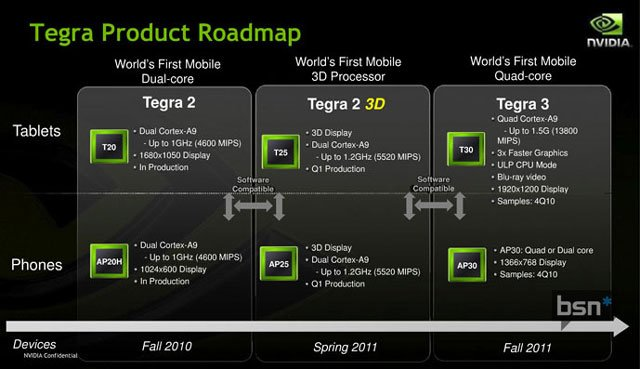
\includegraphics[width=11.0cm]{./pictures/EvolucaoTegra.png}
  %\end{figure}
\end{frame}


\section{Introdu\c{c}\~ao}
\begin{frame}{Introdu\c{c}\~ao}
  \begin{itemize}
    \item Por que Multi Porcessamento
    \begin{itemize}
      \item Aplica\c{c}\~oes mais robustas
      \item Menor consumo de energia
      \begin{itemize}
	\item Opera em frequ\^encias menores
	\item Opera por menos tempo na frequ\^encia de pico
      \end{itemize}
    \item Mais Eficiente
    \begin{itemize}
      \item Realiza tarefas simultaneamente
    \end{itemize}
   \end{itemize}
  \end{itemize}
\end{frame}

\section{Caracter\'isticas}

\subsection{Propriedades}
\begin{frame}
  \begin{table}
    \centering
    \caption{Caracter\'isticas dos Tegra 2 e 3}
    \begin{tabular}{|p{5cm}|p{5cm}|}
      \hline
      Tegra 2 & Tegra 3 \\
      \hline
      \multicolumn{2}{|c|}{Processador} \\
      \hline
      DualCore  & QuadCore mais n\'ucleo econ\^omico \\
      \hline
      Acima de 1.2 GHz  & Acima de 1.5 GHz - SingleCore/Acima de 1.4 Ghz - QuadCore \\
      \hline
      \multicolumn{2}{|c|}{Cache  L1(I/D)} \\
      \hline
      32KB/32KB por n\'ucleo & 32KB/32KB por n\'ucleo \\
      \hline
      \multicolumn{2}{|c|}{Cache  L2} \\
      \hline
      1 MB & 1 MB\\
      \hline
      \multicolumn{2}{|c|}{Mem\'oria} \\
      \hline
      Acima de 1 GB & Acima de 2 GB\\
      \hline
    \end{tabular}
  \end{table}
\end{frame}

\begin{frame}
 \begin{table}
    \centering
    \caption{Caracter\'isticas dos Tegra 2 e 3}
    \begin{tabular}{|p{5cm}|p{5cm}|}
      \hline
      Tegra 2 & Tegra 3 \\
      \hline
      \multicolumn{2}{|c|}{Arquitetura GPU} \\
      \hline
      GPU GeForce ULP & GeForce ULP\\
      \hline
      \multicolumn{2}{|c|}{Performance 3D} \\
      \hline
      1x & 3X\\
      \hline
      \multicolumn{2}{|c|}{N\'ucleos GPU} \\
      \hline
      8 & 12\\
      \hline     
    \end{tabular}
  \end{table}
\end{frame}


\subsection{Benchmarks}  
\begin{frame}
  \begin{figure}[ht]
    \centering
    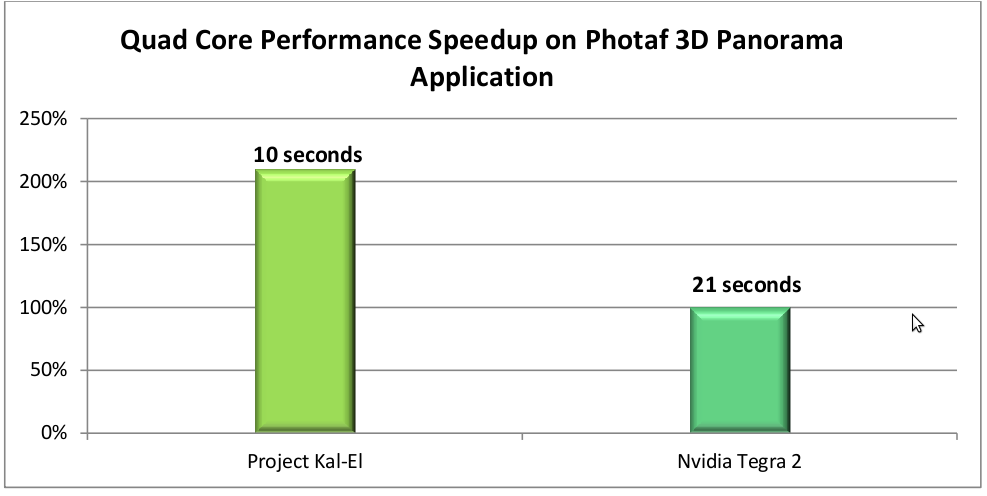
\includegraphics[width=10.0cm]{./pictures/QuadCorePhota.png}
   \end{figure}
\end{frame}

\begin{frame}
  \begin{figure}[ht]
    \centering
    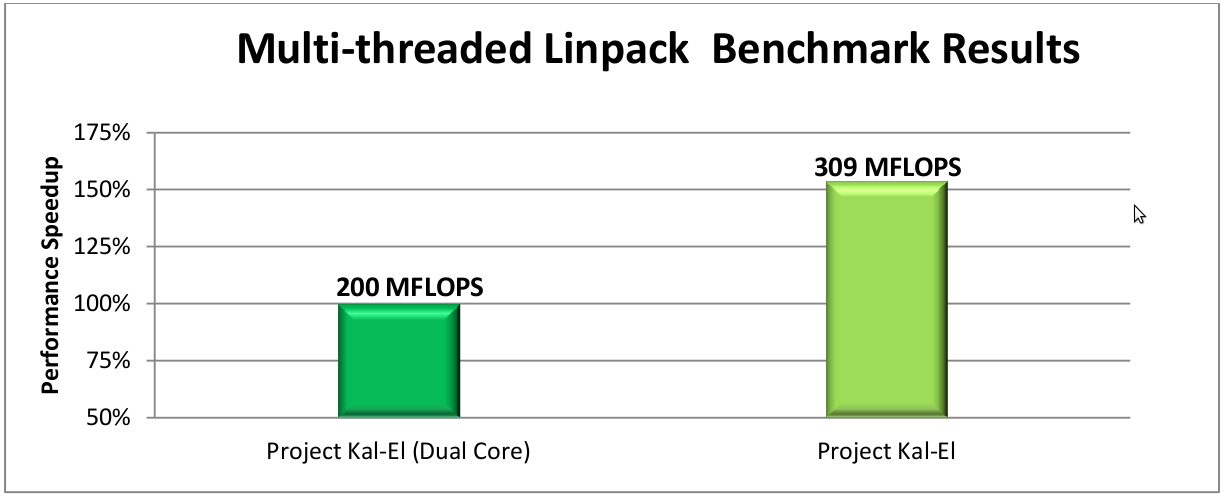
\includegraphics[width=10.0cm]{./pictures/MultiThread.png}
  \end{figure}
\end{frame}

\begin{frame}
  \begin{figure}[ht]
    \centering
    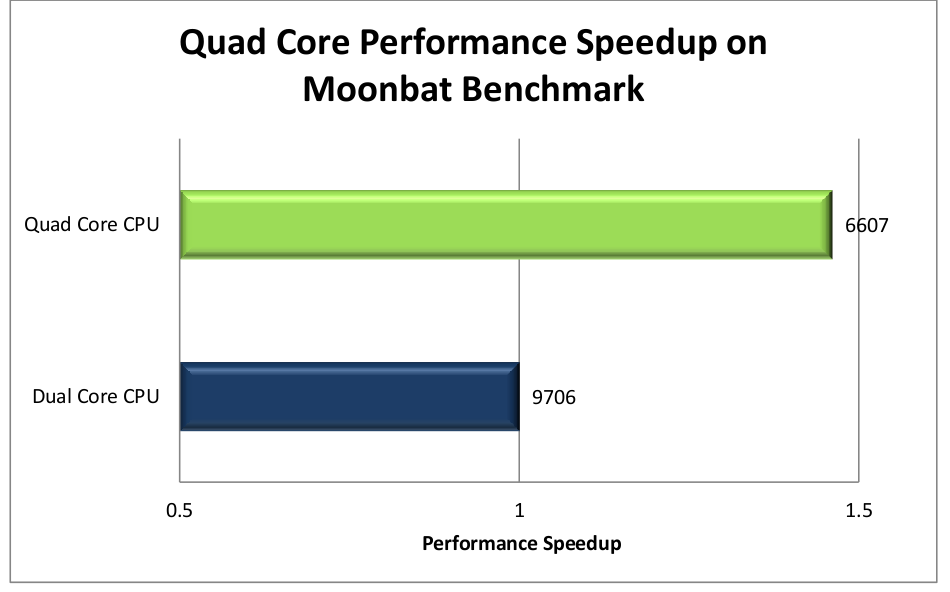
\includegraphics[width=10.0cm]{./pictures/QuadCoreBenchmark.png}
  \end{figure}
\end{frame}

\begin{frame}
  \begin{figure}[ht]
    \centering
    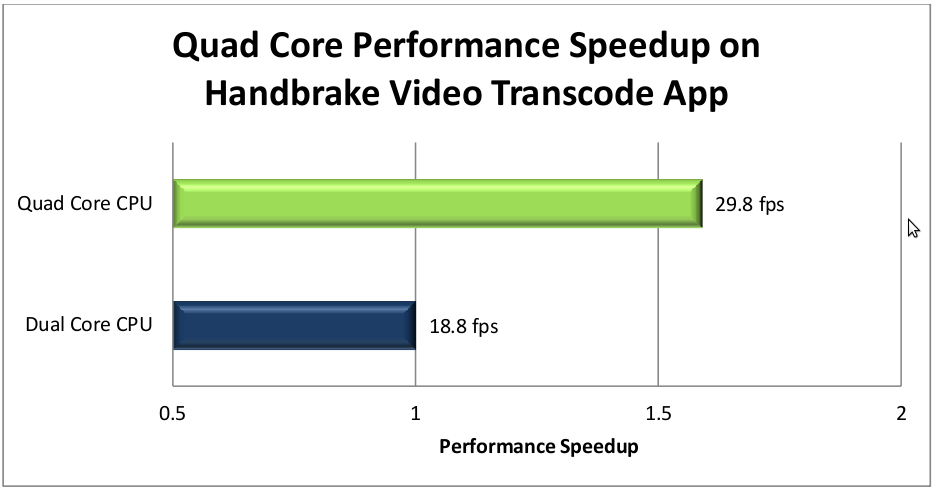
\includegraphics[width=10.0cm]{./pictures/QuadCoreVideo.png}
  \end{figure}
\end{frame}
    
    
\subsection{Processo de fabrica\c{c}\~ao X Consumo}
 \begin{frame}
  \begin{itemize}
    \item Consumo
    \begin{itemize}
      \item \( (ET)\ =\ (EF)\ +\ (ED) \)
      \item \( (ED)\  \alpha\  f(V)^2\)
    \end{itemize}
  \end{itemize}
\end{frame}
  
\begin{frame}
  \begin{itemize}
    \item Tecnologias usadas para fabrica\c{c}\~ao do chip sil\'icio
    \begin{itemize}
      \item Tecnologia de processo r\'apido
      \begin{itemize}
	\item Maior EV
	\item Menor tempo de troca
      \end{itemize}
    \end{itemize}
    \begin{itemize}
      \item Tecnologia de processo de baixa pot\^encia
      \begin{itemize}
	\item Menor EV
	\item Maior tempo de troca
      \end{itemize}
    \end{itemize}
  \end{itemize}
\end{frame}

\begin{frame}
  \begin{figure}[ht]
    \centering
    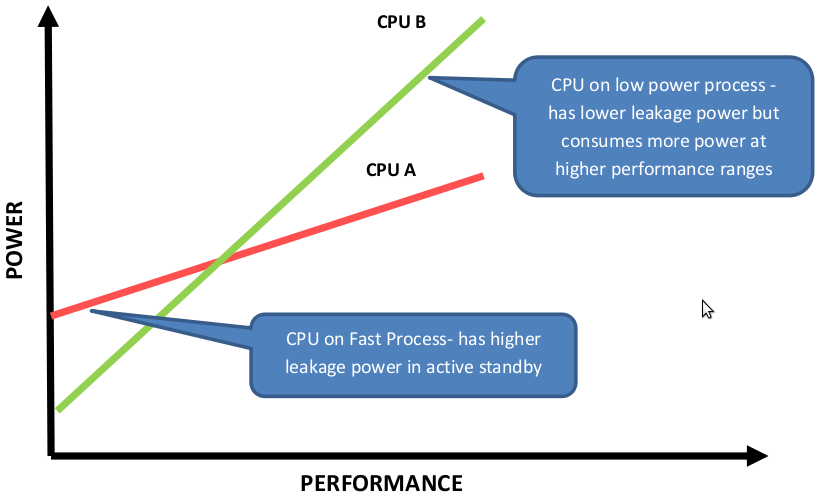
\includegraphics[width=8.5cm]{./pictures/Tecnologiasdeprocesso.png}
  \end{figure}
\end{frame}
   
\subsection{Arquitetura vSMP}
\begin{frame}
  \begin{itemize}
  \item Multi Processamento Sim\'etrico vari\'avel
    \begin{itemize}
      \item 4 n\'ucleos principais
      \item 1 Companion Core (at\'e 500 Mhz)
      \item Combina\c{c}\~ao dos dois processos de fabrica\c{c}\~ao
    \end{itemize}
  \end{itemize}
  \begin{figure}
    \centering
    \includegraphics[width=6.8cm]{./pictures/CompanionCore}
  \end{figure}
\end{frame}

\begin{frame}
  \centering
  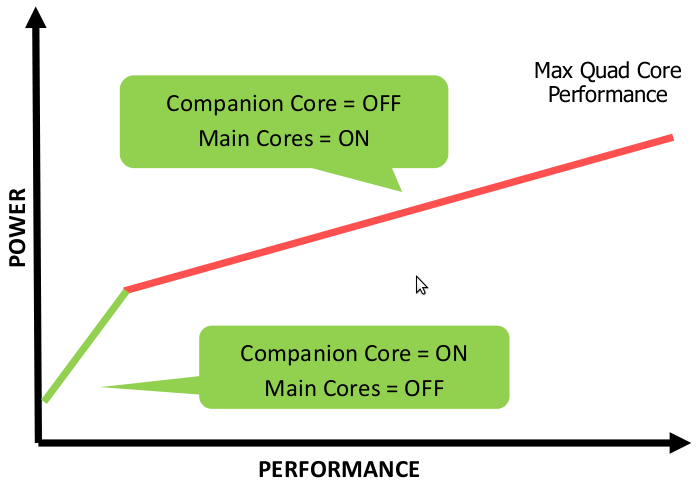
\includegraphics[width=10.0cm]{./pictures/vSMP}
\end{frame}

\subsubsection{Vantagens}
\begin{frame}
  \begin{itemize}
    \item Vantagens
    \begin{itemize}
      \item Transpar\^encia para o SO
      \begin{itemize}
	\item Monitoramento do workload das CPU's
	\item A pr\'opria arquitetura faz a troca dos processadores
      \end{itemize}
      \item Coer\^encia de Cache
      \begin{itemize}
	\item Sincroniza\c{c}\~ao de mem\'oria cache
	\item N\'ucleos compartilham a mesma cache L2
	\item Os n\'ucleos principais n\~ao podem atuar junto com o Companion Core
      \end{itemize}
    \end{itemize}
  \end{itemize}
\end{frame}
  
\begin{frame}
  \begin{figure}
    \centering
    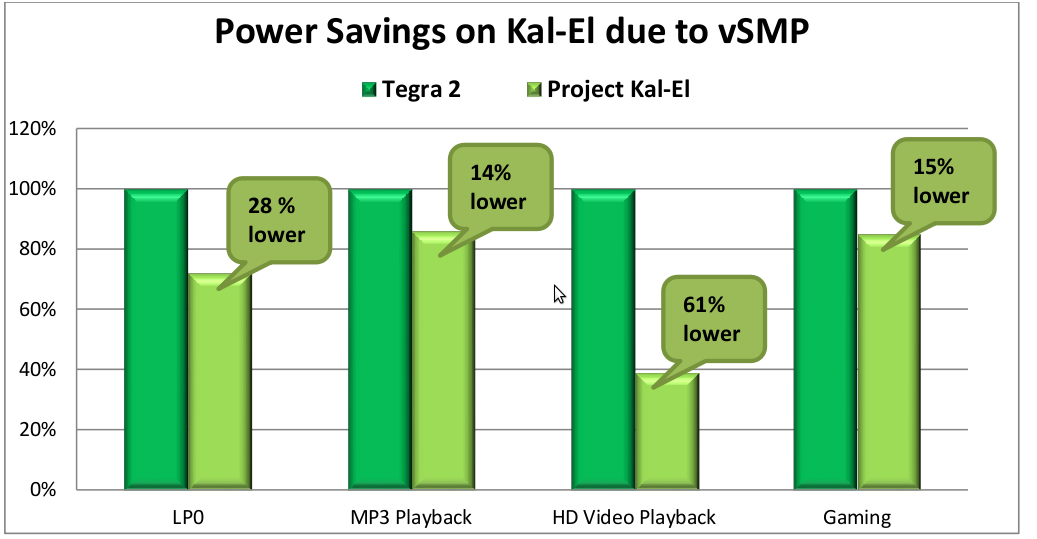
\includegraphics[width=10.0cm]{./pictures/PowerSavesVSMP}
  \end{figure}
\end{frame}

\begin{frame}
  \begin{figure}
    \centering
    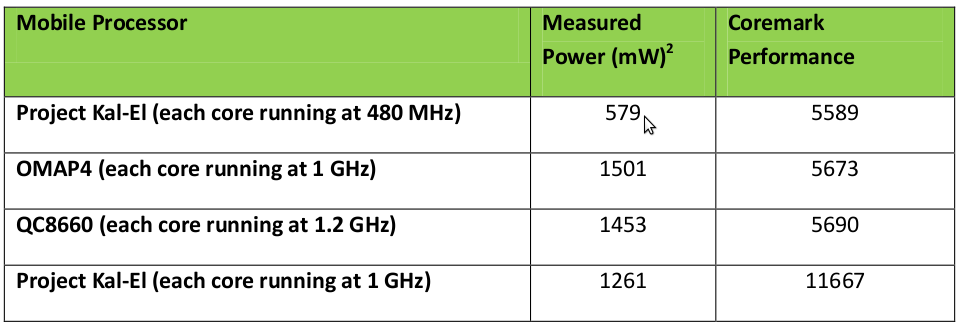
\includegraphics[width=10.0cm]{./pictures/Table1}
  \end{figure}
\end{frame}

\begin{frame}
  \begin{figure}
    \centering
    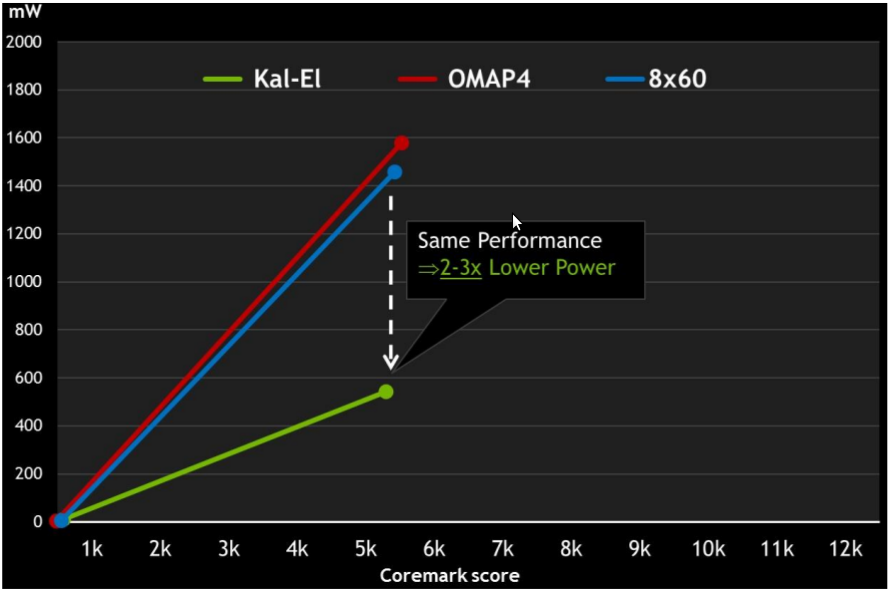
\includegraphics[width=10.0cm]{./pictures/Kal-ElLowerFrequency}
  \end{figure}
\end{frame}

\begin{frame}
  \begin{figure}
    \centering
    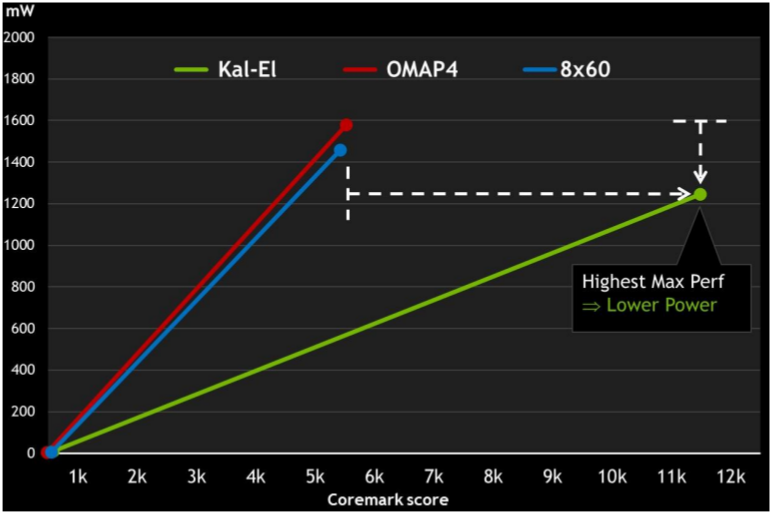
\includegraphics[width=10.0cm]{./pictures/Kal-ElHigherFrequency}
  \end{figure}
\end{frame}

\section{Aplica\c{c}\~oes}
\begin{frame}
  \begin{itemize}
    \item Smatphones
    \item Tablets
  \end{itemize}
  \begin{figure}
    \centering
    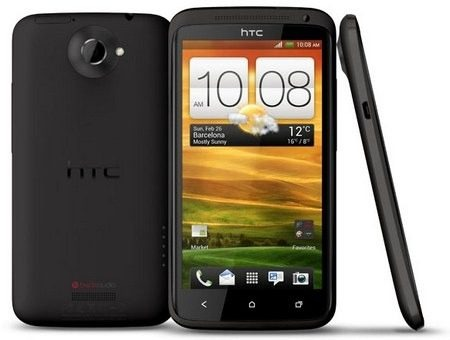
\includegraphics[width=9.0cm]{./pictures/htcTegra3.png}
  \end{figure}
\end{frame}

    
\end{document}
